% !TeX root = report_example.tex
\newcommand*{\PathToAssets}{../assets}%
\newcommand*{\PathToOutput}{../_output}%
% \newcommand*{\PathToBibFile}{bibliography.bib}%


%%%%%%%%%%%%%%%%%%%%%%%%%%%%%%%%%%%%%%
%% This file is compiled with XeLaTex.
%%%%%%%%%%%%%%%%%%%%%%%%%%%%%%%%%%%%%%
\documentclass[12pt]{article}
%\documentclass[reqno]{amsart}
%\documentclass[titlepage]{amsart}
\usepackage{my_article_header}
\usepackage{my_common_header}

\begin{document}
\title{
Insert Title Here
\\{\color{blue} \large Preliminary Idea Write-up}
}
% {\color{blue} \large Preliminary. Do not distribute.}
% }

\author{
Insert Authors Here\footnote{Author affiliation}
  % \newline 
  % \hspace{3pt} \indent \hspace{3pt}
  % % I am immensely grateful to...
}
% \maketitle
\begin{titlepage}
% \input{cover_letter.tex}
\maketitle
%http://tex.stackexchange.com/questions/141446/problem-of-duplicate-identifier-when-using-bibentry-and-hyperref
% \nobibliography*

% Abstract should have fewer than 150 words

\doublespacing
\begin{abstract}
Lorem ipsum dolor sit amet, consectetur adipiscing elit, sed do eiusmod tempor
incididunt ut labore et dolore magna aliqua. Ut enim ad minim veniam, quis
nostrud exercitation ullamco laboris nisi ut aliquip ex ea commodo consequat.
Duis aute irure dolor in reprehenderit in voluptate velit esse cillum dolore
eu fugiat nulla pariatur. Excepteur sint occaecat cupidatat non proident,
sunt in culpa qui officia deserunt mollit anim id est laborum.
\end{abstract}


\end{titlepage}

\doublespacing
\section{Introduction}

Accumsan lacus vel facilisis volutpat est velit egestas. Nisi quis eleifend
quam adipiscing. Turpis egestas pretium aenean pharetra magna ac placerat.
Nec tincidunt praesent semper feugiat nibh. Sapien et ligula ullamcorper
malesuada. Ac turpis egestas integer eget aliquet nibh praesent. Purus in
massa tempor nec feugiat nisl pretium. Et sollicitudin ac orci phasellus
egestas tellus rutrum tellus pellentesque. Aliquet nibh praesent tristique
magna sit. Sem et tortor consequat id.


\begin{textbox}{green}{Comments}
Here is a textbox...
\end{textbox}

I give an example of a simple table in Table \ref{table:pandas_to_latex_simple_table1.tex}.


\begin{table}
\caption{A Simple Table From Pandas, No. 1}
\centering
\input{\PathToOutput/pandas_to_latex_simple_table1.tex}
\caption*{
  Here I show some data...
}
\label{table:pandas_to_latex_simple_table1.tex}
\end{table}


\section{Model}

The Black–Scholes equation governing the price evolution of derivatives under
the Black–Scholes model is given in (\ref{eq:black-scholes}). Some aligned
equations are given in (\ref{eq:align1}) and (\ref{eq:align2}). I give an
example in which the two share a single equation number in
(\ref{eq:align-share}). Be sure to take a look at the results in 
Table \ref{table:example_table.tex} and the diagram in 
Figure \ref{fig:star_network_n_nodes.eps}.
Arcu felis bibendum ut tristique et. Eget gravida
cum sociis natoque penatibus et magnis. Elit pellentesque habitant morbi
tristique senectus et netus et.
\todo[inline]{This is an inline TODO note} 
Nunc sed blandit libero volutpat.
Potenti nullam ac tortor vitae purus faucibus. Turpis massa sed elementum
tempus. Aliquet eget sit amet tellus. Pharetra convallis posuere morbi leo
urna molestie at. Massa ultricies mi quis hendrerit dolor magna. Elit
pellentesque habitant morbi tristique senectus et netus et malesuada. In
hendrerit gravida rutrum quisque. Facilisi cras fermentum odio eu.
Pellentesque elit ullamcorper dignissim cras tincidunt. Lacinia at quis
risus sed vulputate odio ut enim. 
\todo{This is a TODO in the margin.}

\begin{equation}
\frac{\partial V}{\partial t} + \frac{1}{2}\sigma^2 S^2 \frac{\partial^2 V}{\partial S^2} 
+ rS\frac{\partial V}{\partial S} - rV = 0
\label{eq:black-scholes}
\end{equation}

Accumsan lacus vel facilisis volutpat est velit egestas. Nisi quis eleifend
quam adipiscing. Turpis egestas pretium aenean pharetra magna ac placerat.
Nec tincidunt praesent semper feugiat nibh. Sapien et ligula ullamcorper
malesuada. Ac turpis egestas integer eget aliquet nibh praesent. Purus in
massa tempor nec feugiat nisl pretium. Et sollicitudin ac orci phasellus
egestas tellus rutrum tellus pellentesque. Aliquet nibh praesent tristique
magna sit. Sem et tortor consequat id.

\begin{align}
P(S_t, t) &= Ke^{-r(T - t)} - S_t + C(S_t, t)   \label{eq:align1}\\
          &= N(-d_-) Ke^{-r(T - t)} - N(-d_+) S_t \label{eq:align2}
\end{align}



\begin{table}
\caption{Summary Stats}
\centering
\input{\PathToOutput/example_table.tex}
\caption*{
  Here I show some data...
}
\label{table:example_table.tex}
\end{table}

\begin{align}
\begin{split}
P(S_t, t) &= Ke^{-r(T - t)} - S_t + C(S_t, t)   \\
          &= N(-d_-) Ke^{-r(T - t)} - N(-d_+) S_t 
\end{split}
\label{eq:align-share}
\end{align}



Vitae congue mauris rhoncus aenean. Turpis egestas pretium aenean pharetra.
Non pulvinar neque laoreet suspendisse interdum consectetur libero id
faucibus. Id porta nibh venenatis cras sed. Viverra tellus in hac habitasse
platea. Sit amet facilisis magna etiam tempor orci eu lobortis elementum.
Porttitor leo a diam sollicitudin. Imperdiet proin fermentum leo vel orci
porta non. Maecenas pharetra convallis posuere morbi. Vel risus commodo
viverra maecenas accumsan lacus vel facilisis volutpat. Faucibus vitae
aliquet nec ullamcorper sit amet risus nullam. Sit amet venenatis urna cursus
eget nunc scelerisque viverra mauris. A arcu cursus vitae congue. Ullamcorper
morbi tincidunt ornare massa eget.

\begin{figure}
\centering
\captionsetup{width=0.8\textwidth}
\caption{Network}
  \centering
  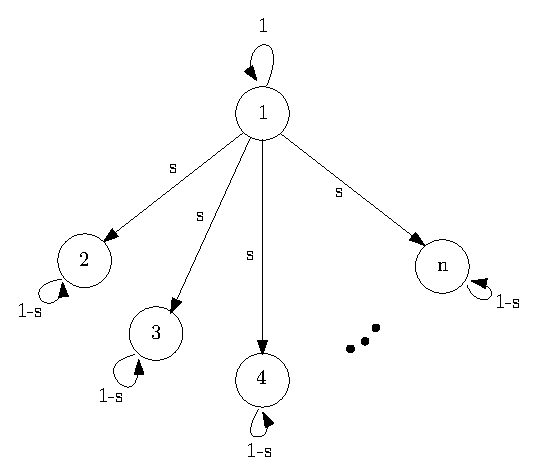
\includegraphics[width=0.6\linewidth]{\PathToAssets/star_network_n_nodes.eps}
\caption*{
  Star network
  }
\label{fig:star_network_n_nodes.eps}
\end{figure}


Eget duis at tellus at. Turpis egestas integer eget aliquet nibh praesent
tristique magna. Egestas diam in arcu cursus euismod quis viverra nibh cras.
Velit laoreet id donec ultrices tincidunt arcu non sodales. Urna duis
convallis convallis tellus id. Ut pharetra sit amet aliquam. Adipiscing
commodo elit at imperdiet dui accumsan sit. Arcu cursus euismod quis viverra
nibh. Dictum at tempor commodo ullamcorper a. Nunc eget lorem dolor sed
viverra. Pellentesque pulvinar pellentesque habitant morbi tristique senectus
et netus et. Feugiat pretium nibh ipsum consequat nisl vel. Magna fermentum
iaculis eu non diam phasellus vestibulum. Et netus et malesuada fames ac
turpis. Purus ut faucibus pulvinar elementum integer enim neque. Sem
fringilla ut morbi tincidunt augue. Facilisi cras fermentum odio eu feugiat
pretium nibh. Pellentesque nec nam aliquam sem et. Mi bibendum neque egestas
congue quisque egestas diam. For example, see \citet{fama1992cross}. Also, here's another
way to cite \citep{sharpe1964capital}.

\begin{figure}
\centering
\caption{Example plot}
  \centering
  \includegraphics[width=0.75\linewidth]{\PathToOutput/example_plot.png}
  % \caption{Average returns}
\caption*{
  Inflation and Real GDP...
  }
\label{fig:div-futures-habits-comparison}
\end{figure}

Enim sit amet venenatis urna cursus eget. Dictumst quisque sagittis purus sit
amet volutpat consequat mauris. Accumsan sit amet nulla facilisi morbi tempus
iaculis urna id. Vel turpis nunc eget lorem dolor. Rutrum quisque non tellus
orci ac auctor augue mauris. Vestibulum mattis ullamcorper velit sed
ullamcorper morbi. In fermentum posuere urna nec tincidunt. Mollis nunc sed
id semper risus in hendrerit gravida rutrum. Ante in nibh mauris cursus
mattis molestie a iaculis at. Consectetur a erat nam at. Ac turpis egestas
integer eget aliquet nibh praesent tristique. Et netus et malesuada fames ac.
Mollis nunc sed id semper risus in hendrerit gravida. Platea dictumst quisque
sagittis purus.

\begin{mydefinition}[Fibration]
  A fibration is a mapping between two topological spaces that has the homotopy lifting property for every space \(X\).
\end{mydefinition}

\begin{proposition}
  Let \(f\) be a function whose derivative exists in every point, then \(f\) is 
  a continuous function.
\end{proposition}
\begin{proof}
  We have that \(f\) is a differentiable function and so it must be continuous.
\end{proof}

\begin{mylemma}
  Given two line segments whose lengths are \(a\) and \(b\) respectively there is a 
  real number \(r\) such that \(b=ra\).
\end{mylemma}

\begin{proof}
  To prove it by contradiction try and assume that the statement is false,
  proceed from there and at some point you will arrive to a contradiction.
\end{proof}

Ac turpis egestas maecenas pharetra convallis posuere. Vitae aliquet nec
ullamcorper sit amet risus nullam. Feugiat nisl pretium fusce id velit ut
tortor pretium. Nec ullamcorper sit amet risus nullam eget felis eget nunc.
Luctus accumsan tortor posuere ac ut consequat semper viverra nam. Egestas
pretium aenean pharetra magna. Pharetra massa massa ultricies mi quis
hendrerit dolor. Est ullamcorper eget nulla facilisi etiam dignissim diam.
Sagittis vitae et leo duis ut diam quam. Magna ac placerat vestibulum lectus
mauris ultrices eros in cursus. Adipiscing diam donec adipiscing tristique
risus nec feugiat in. Sed pulvinar proin gravida hendrerit.

Magna eget est lorem ipsum dolor. Id ornare arcu odio ut sem nulla pharetra.
Imperdiet massa tincidunt nunc pulvinar sapien et ligula. Vulputate odio ut
enim blandit volutpat maecenas volutpat blandit aliquam. Turpis egestas
integer eget aliquet nibh praesent tristique magna. Diam phasellus vestibulum
lorem sed risus ultricies tristique nulla. Augue lacus viverra vitae congue
eu. Lacus laoreet non curabitur gravida. Iaculis urna id volutpat lacus
laoreet. Mi in nulla posuere sollicitudin aliquam ultrices sagittis. Enim
nunc faucibus a pellentesque sit amet porttitor eget. Aliquam sem fringilla
ut morbi tincidunt augue interdum velit euismod. Pellentesque massa placerat
duis ultricies lacus sed.

Et tortor consequat id porta. Nam libero justo laoreet sit amet cursus sit. A
iaculis at erat pellentesque adipiscing commodo elit. Pharetra vel turpis
nunc eget. Turpis nunc eget lorem dolor sed viverra ipsum nunc aliquet. Quam
adipiscing vitae proin sagittis. Vitae suscipit tellus mauris a diam maecenas
sed enim ut. Rutrum tellus pellentesque eu tincidunt. Pellentesque diam
volutpat commodo sed. Erat velit scelerisque in dictum non. Consectetur lorem
donec massa sapien faucibus et molestie. Suspendisse potenti nullam ac
tortor. Amet massa vitae tortor condimentum lacinia quis. Et malesuada fames
ac turpis egestas maecenas pharetra. Augue eget arcu dictum varius duis at
consectetur lorem.

\newpage
\bibliographystyle{jpe}
\bibliography{bibliography.bib}  % list here all the bibliographies that you need. 
% \bibliography{\PathToBibFile}
% \printbibliography

\newpage
\begin{appendices}
\section{Proofs}

TODO



\section{Recycle Bin}
{\textbf{(Short-term parking spot for material that may be re-used or deleted at a later time)}}


TODO

\end{appendices}
\end{document}
